\subsection{Aimspice results}

After running a few simulations with different voltages and dimmensions we ended up with the prefered parameters in table \ref{tab:MOSFET_parameters}. Note: the some plots have a typo where it says P\_W instead of $W_P$.

\begin{table}[H]
    \centering
    \caption{MOSFET parameters}
    \label{tab:MOSFET_parameters}
    \begin{tabular}{ll}
    \hline
    Parameter & Value \\ \hline
        $V_{DD}$& 0.6V  \\
        $W_N$ & 100nm \\
        $L_N$ & 100nm \\
        $W_P$ & 300nm \\
        $L_P$ & 100nm     
    \end{tabular}
\end{table}

The static leakage power can be seen in the bargraphs on figure \ref{fig:static_leakage_power_bar}.

\begin{figure}[H]
    \centering
    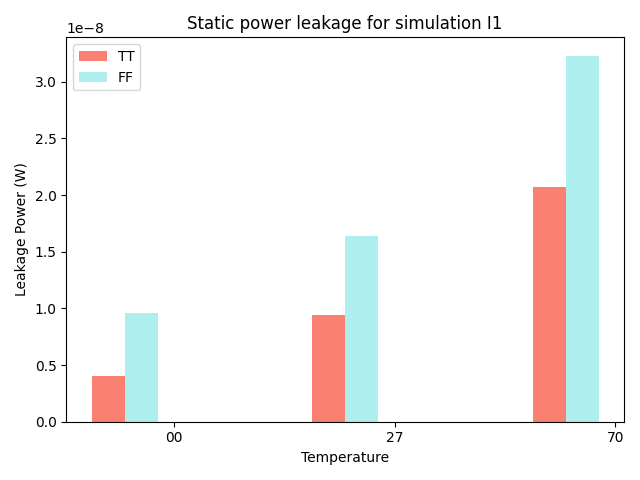
\includegraphics[height= 0.21\textheight]{figures/aimspice/0.600_0.1u_0.1u_0.300u_0.1u/leakage_data/leakage_power_I05.png}
    \vspace{5pt}
    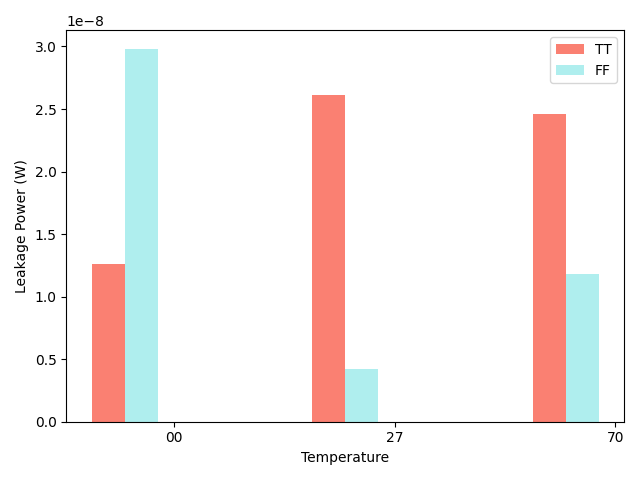
\includegraphics[height= 0.21\textheight]{figures/aimspice/0.600_0.1u_0.1u_0.300u_0.1u/leakage_data/leakage_power_I07.png}
    \vspace{5pt}
    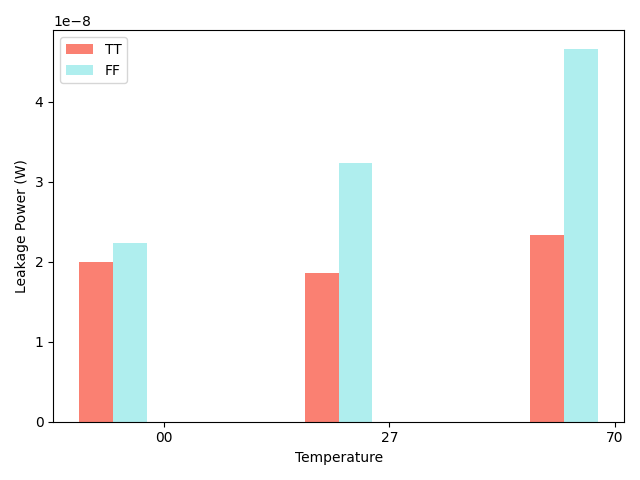
\includegraphics[height= 0.21\textheight]{figures/aimspice/0.600_0.1u_0.1u_0.300u_0.1u/leakage_data/leakage_power_I09.png}
    \vspace{5pt}
    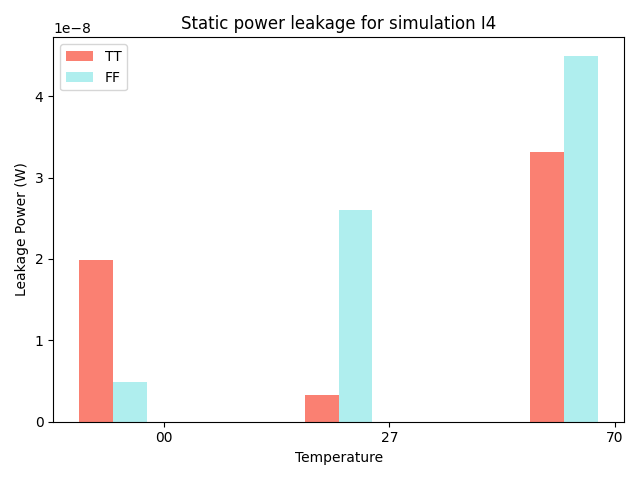
\includegraphics[height= 0.21\textheight]{figures/aimspice/0.600_0.1u_0.1u_0.300u_0.1u/leakage_data/leakage_power_I11.png}
    \vspace{5pt}
    \caption{Computed static leakage power.}
    \label{fig:static_leakage_power_bar}
\end{figure}

The mean of the static leakage power for every scenario I1-I4 are presented in table \ref{tab:leakage_power}.

\begin{table}[H]
    \centering
    \caption{Mean static leakage power}
    \label{tab:leakage_power}
    \begin{tabular}{ccc}
    \hline
    \textbf{Corner} & \textbf{Temperature} & \textbf{Mean Leakage Power} \\
    \hline
    TT & 0  & $1.560 nW$\\
    TT & 27 & $1.278 nW$\\
    TT & 70 & $3.042 nW$\\
    FF & 0  & $1.065 nW$\\
    FF & 27 & $2.243 nW$\\
    FF & 70 & $3.894 nW$\\
    \end{tabular}
\end{table}

The functionality for each corner can be seen on the figures \ref{fig:aimspice_W1_0} to \ref{fig:aimspice_W3_70}

\begin{figure}[H]
    \centering
    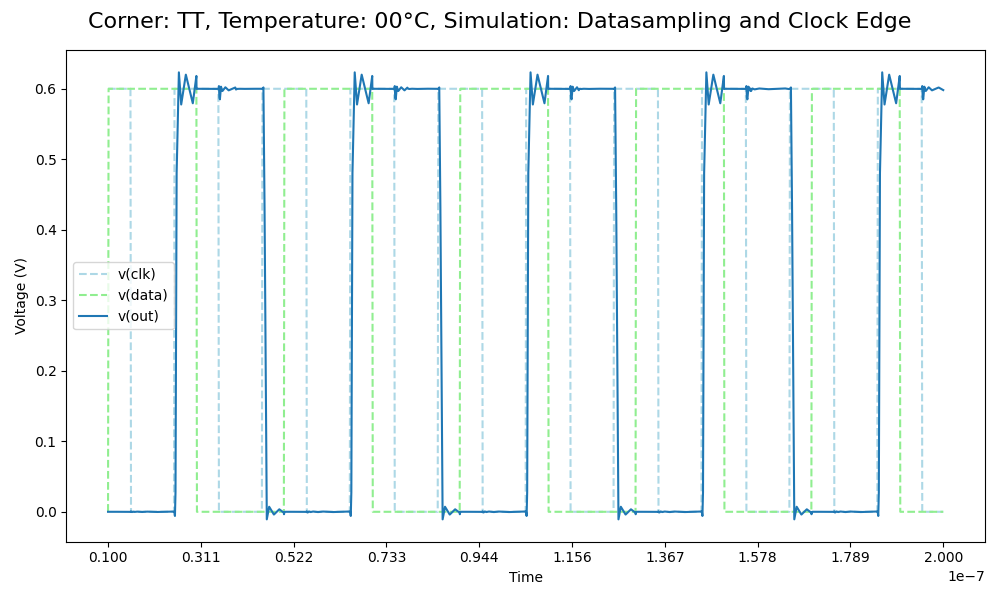
\includegraphics[height= 0.21\textheight]{figures/aimspice/0.600_0.1u_0.1u_0.3u_0.1u/functionality/TT00W1.png}
    \vspace{5pt}
    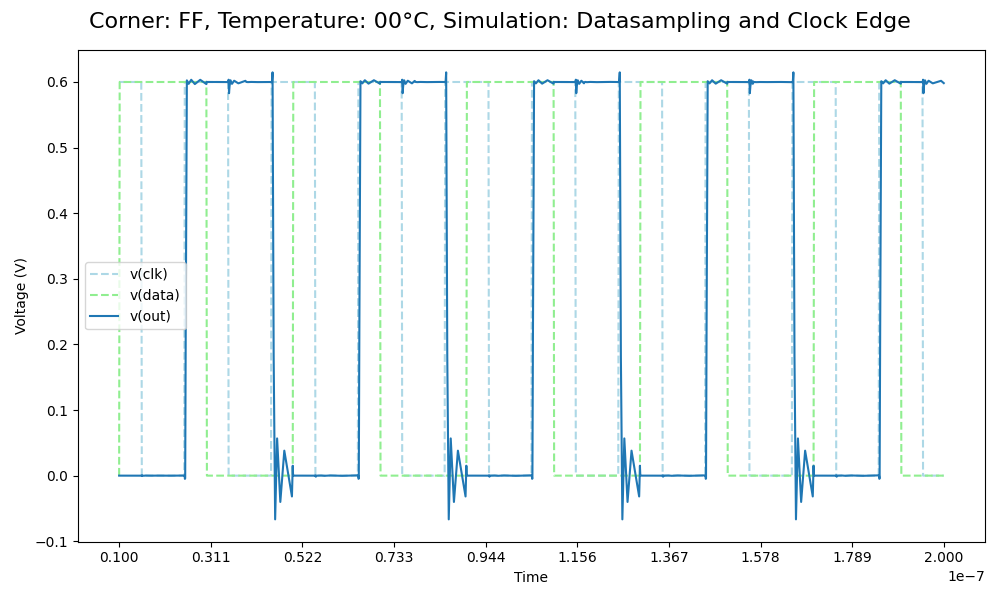
\includegraphics[height= 0.21\textheight]{figures/aimspice/0.600_0.1u_0.1u_0.3u_0.1u/functionality/FF00W1.png}
    \vspace{5pt}
    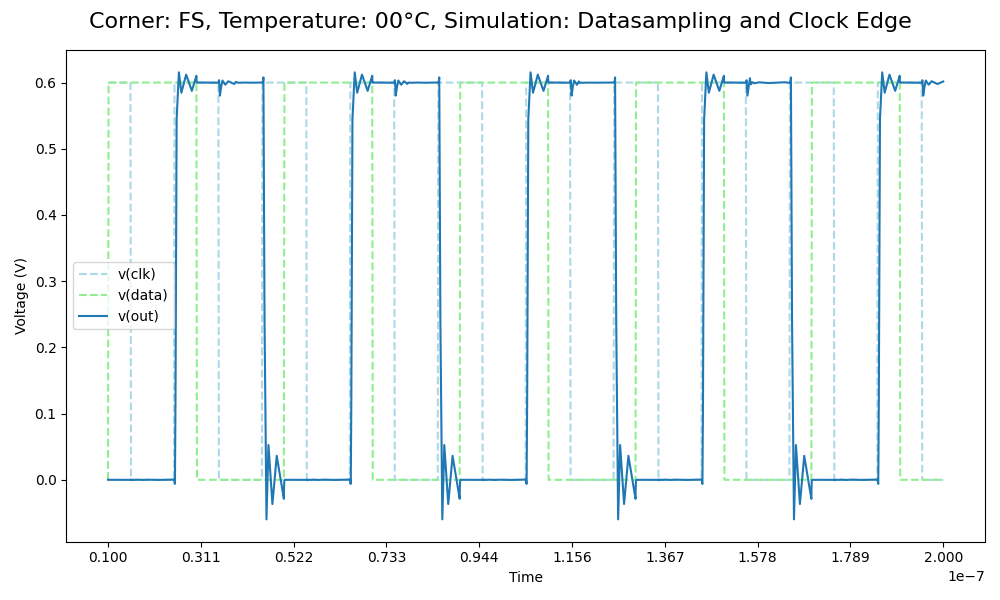
\includegraphics[height= 0.21\textheight]{figures/aimspice/0.600_0.1u_0.1u_0.3u_0.1u/functionality/FS00W1.png}
    \vspace{5pt}
    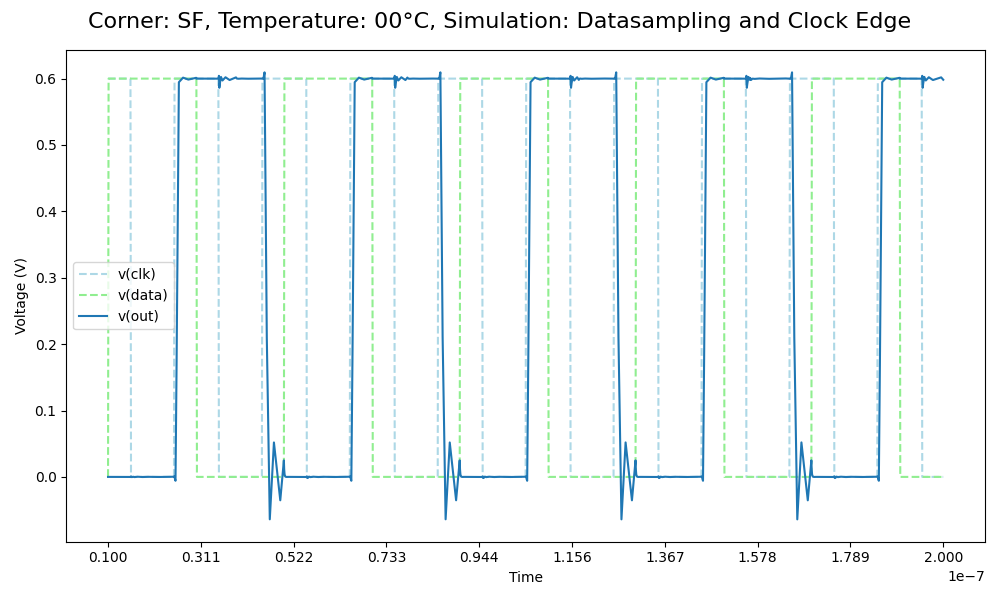
\includegraphics[height= 0.21\textheight]{figures/aimspice/0.600_0.1u_0.1u_0.3u_0.1u/functionality/SF00W1.png}
    \vspace{5pt}
    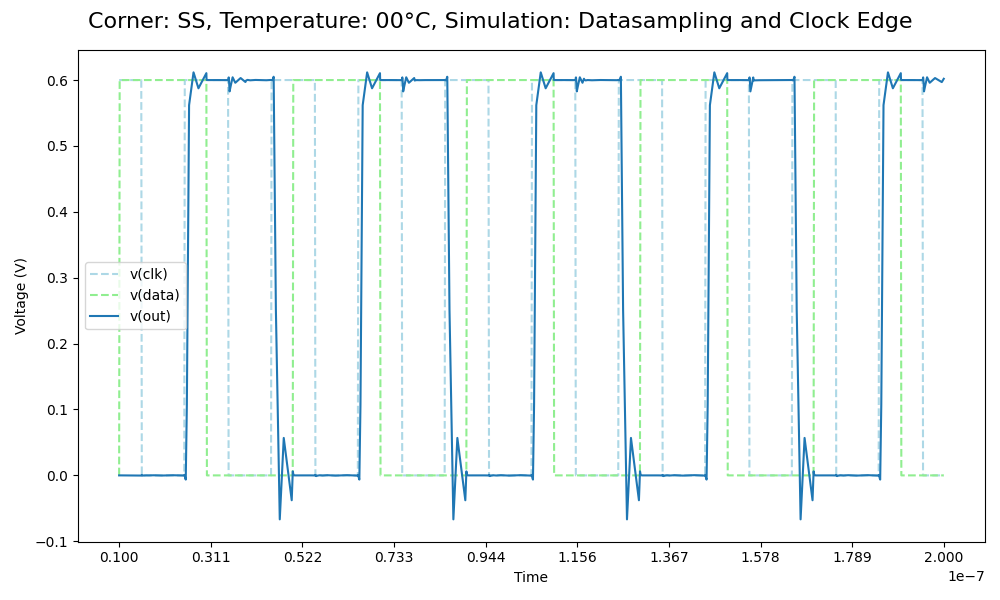
\includegraphics[height= 0.21\textheight]{figures/aimspice/0.600_0.1u_0.1u_0.3u_0.1u/functionality/SS00W1.png}
    \caption{Simulation of datasampling at clock edge at 0 degrees Celsius.}
    \label{fig:aimspice_W1_0}
\end{figure}

\pagebreak

\begin{figure}[H]
    \centering
    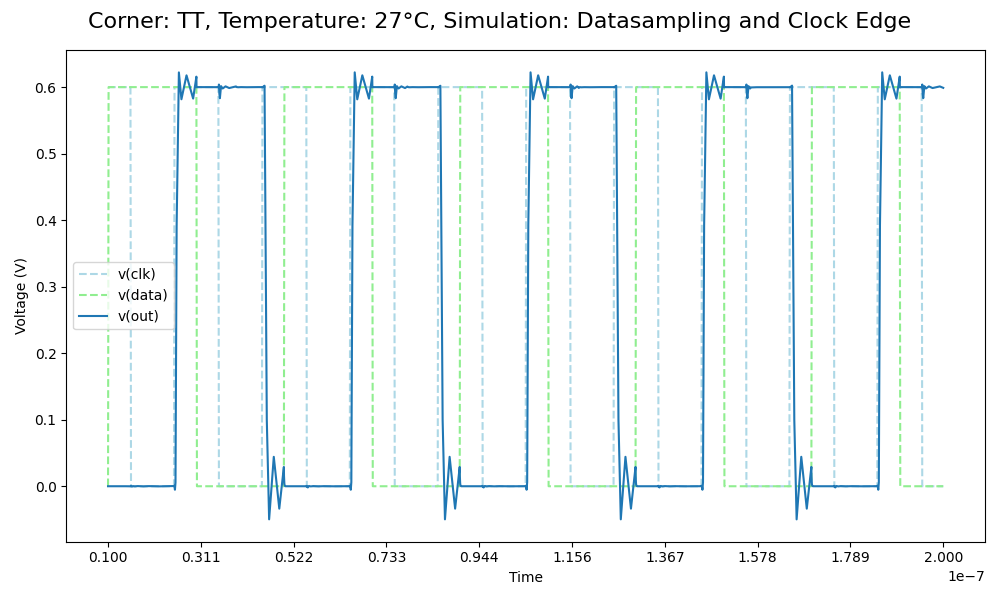
\includegraphics[height= 0.21\textheight]{figures/aimspice/0.600_0.1u_0.1u_0.3u_0.1u/functionality/TT27W1.png}
    \vspace{5pt}
    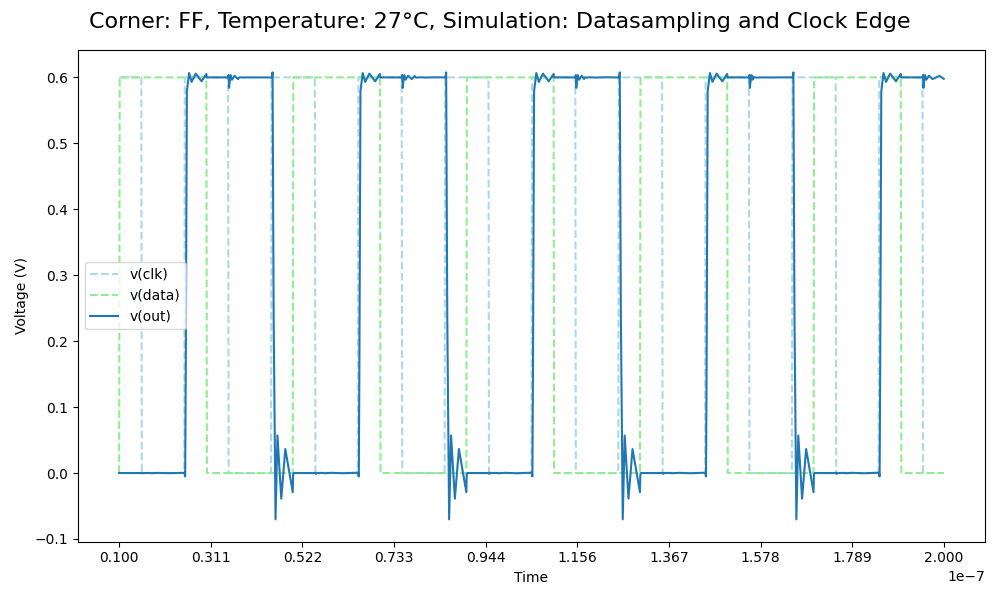
\includegraphics[height= 0.21\textheight]{figures/aimspice/0.600_0.1u_0.1u_0.3u_0.1u/functionality/FF27W1.png}
    \vspace{5pt}
    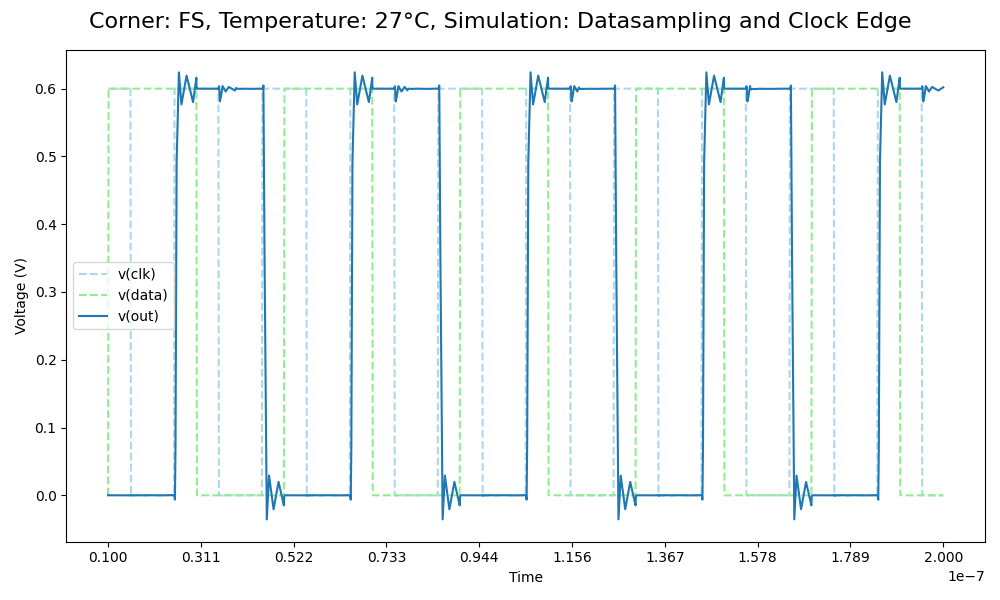
\includegraphics[height= 0.21\textheight]{figures/aimspice/0.600_0.1u_0.1u_0.3u_0.1u/functionality/FS27W1.png}
    \vspace{5pt}
    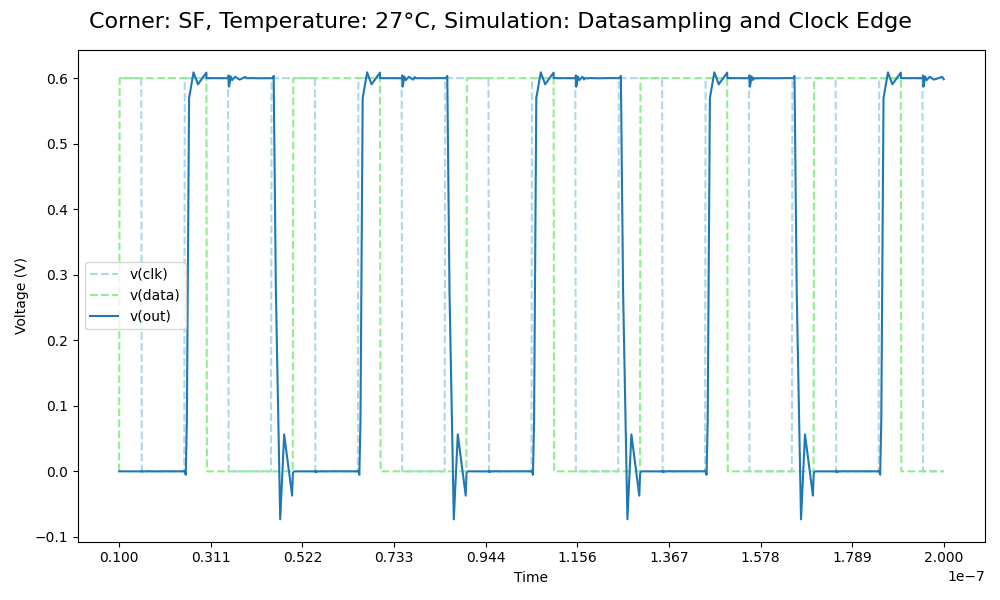
\includegraphics[height= 0.21\textheight]{figures/aimspice/0.600_0.1u_0.1u_0.3u_0.1u/functionality/SF27W1.png}
    \vspace{5pt}
    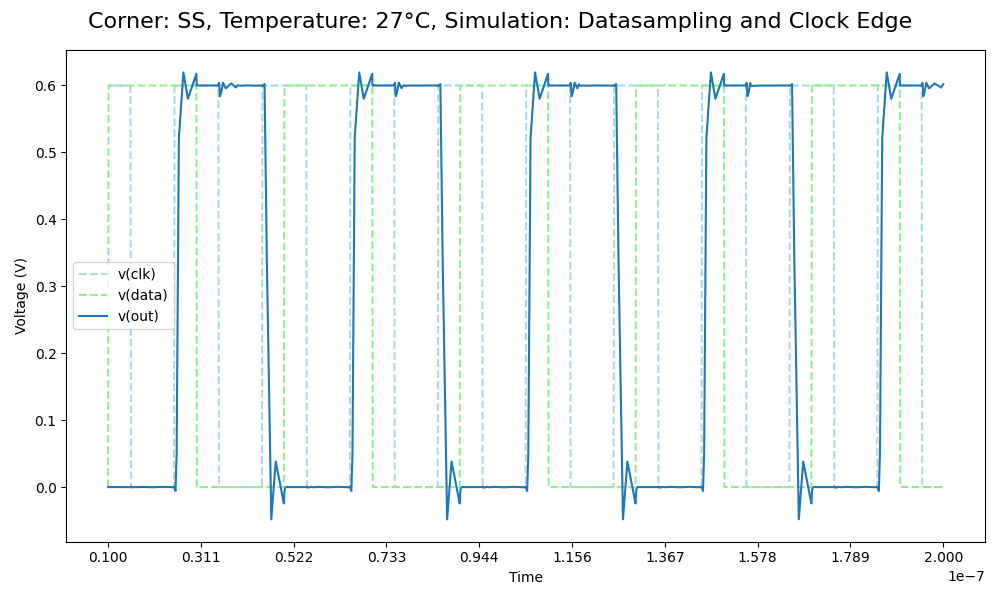
\includegraphics[height= 0.21\textheight]{figures/aimspice/0.600_0.1u_0.1u_0.3u_0.1u/functionality/SS27W1.png}
    \caption{Simulation of datasampling at clock edge at 27 degrees Celsius.}
    \label{fig:aimspice_W1_27}
\end{figure}

\pagebreak

\begin{figure}[H]
    \centering
    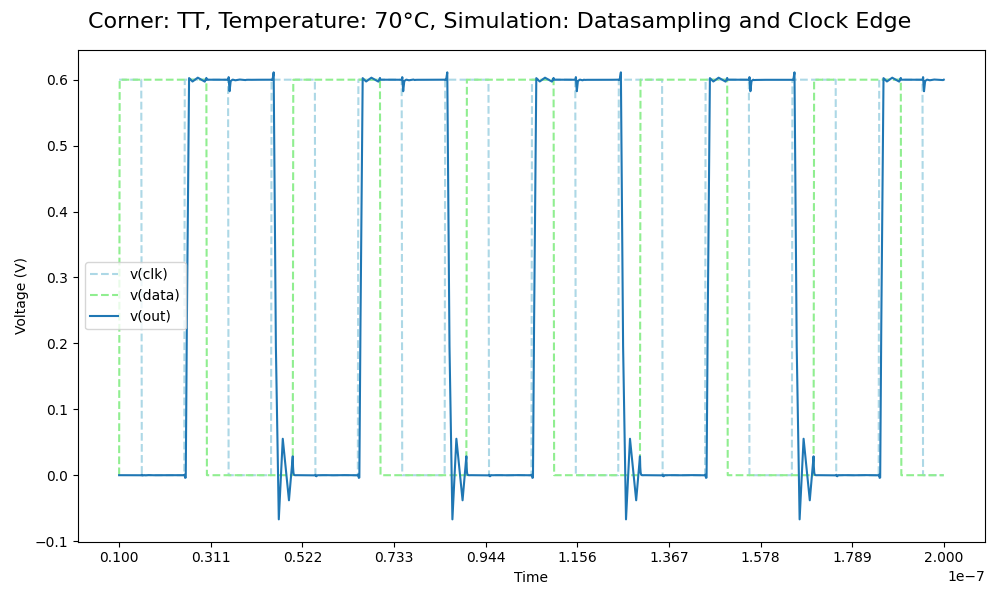
\includegraphics[height= 0.21\textheight]{figures/aimspice/0.600_0.1u_0.1u_0.3u_0.1u/functionality/TT70W1.png}
    \vspace{5pt}
    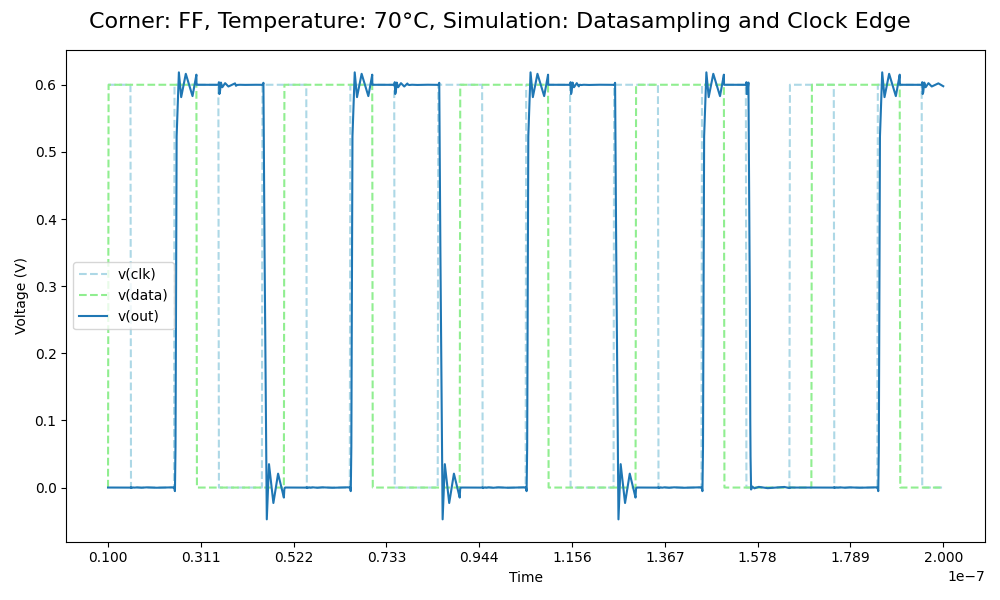
\includegraphics[height= 0.21\textheight]{figures/aimspice/0.600_0.1u_0.1u_0.3u_0.1u/functionality/FF70W1.png}
    \vspace{5pt}
    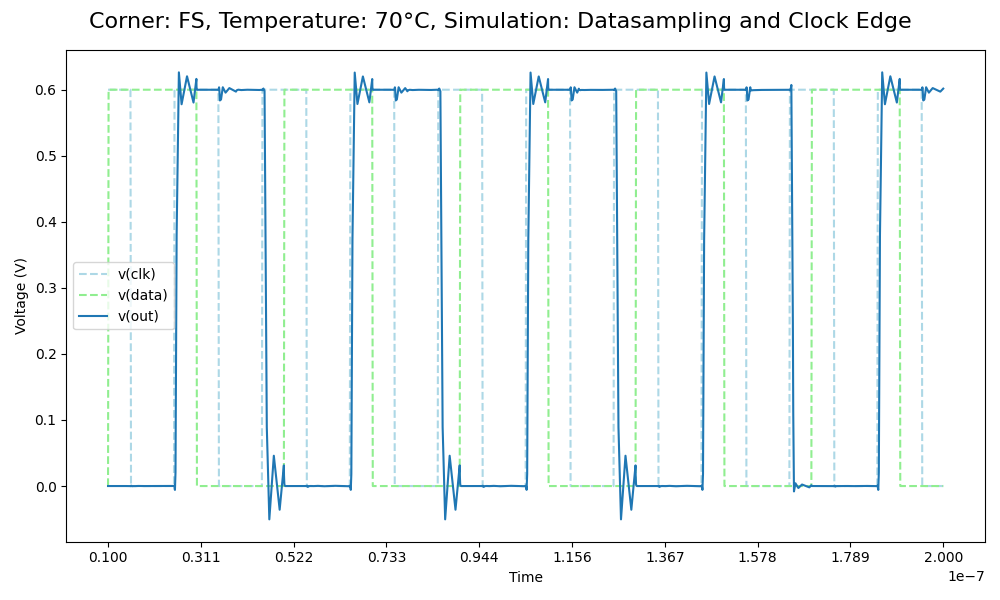
\includegraphics[height= 0.21\textheight]{figures/aimspice/0.600_0.1u_0.1u_0.3u_0.1u/functionality/FS70W1.png}
    \vspace{5pt}
    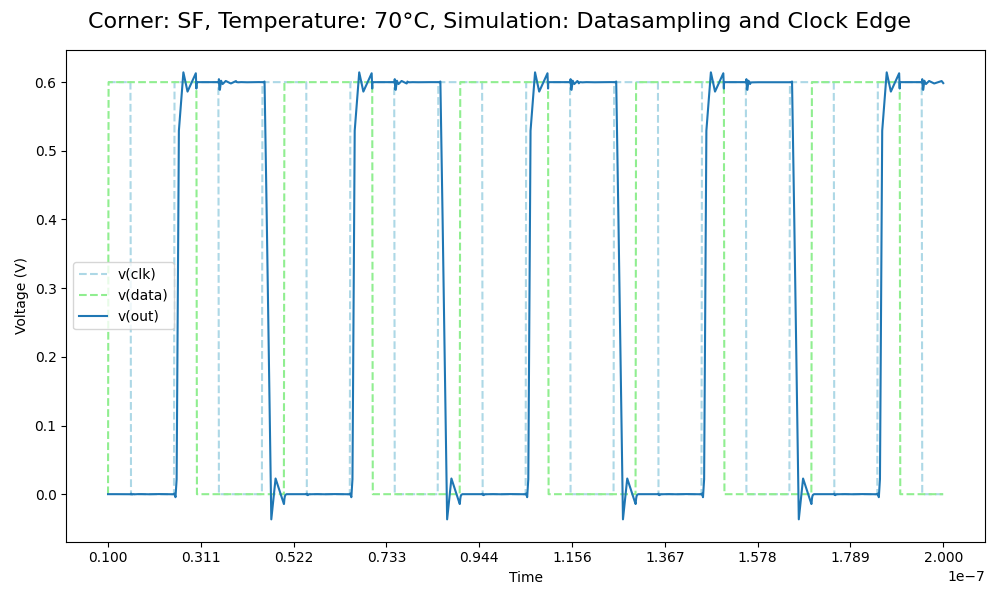
\includegraphics[height= 0.21\textheight]{figures/aimspice/0.600_0.1u_0.1u_0.3u_0.1u/functionality/SF70W1.png}
    \vspace{5pt}
    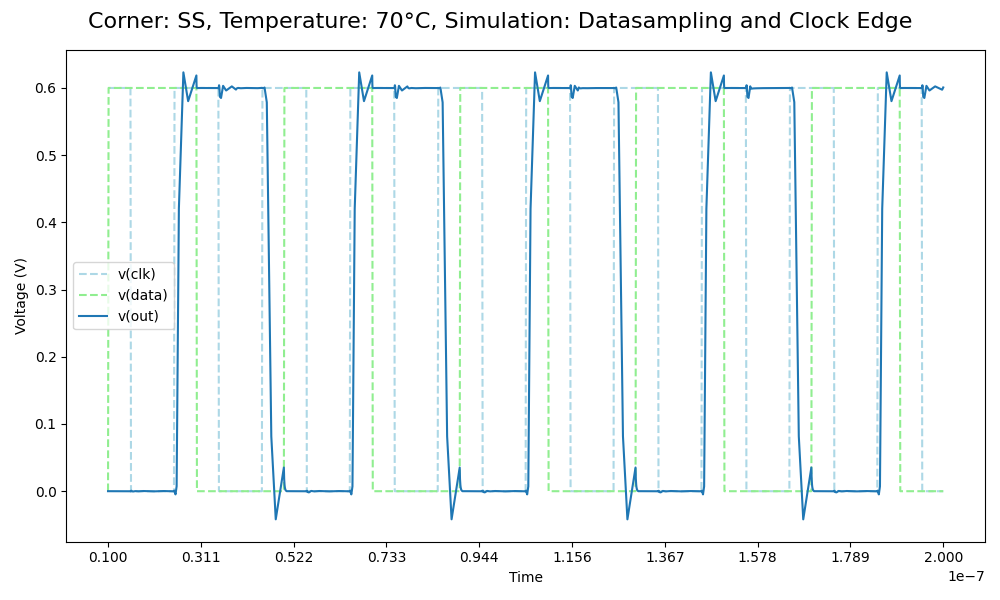
\includegraphics[height= 0.21\textheight]{figures/aimspice/0.600_0.1u_0.1u_0.3u_0.1u/functionality/SS70W1.png}
    \caption{Simulation of datasampling at clock edge at 70 degrees Celsius.}
    \label{fig:aimspice_W1_70}
\end{figure}

\pagebreak

\begin{figure}[H]
    \centering
    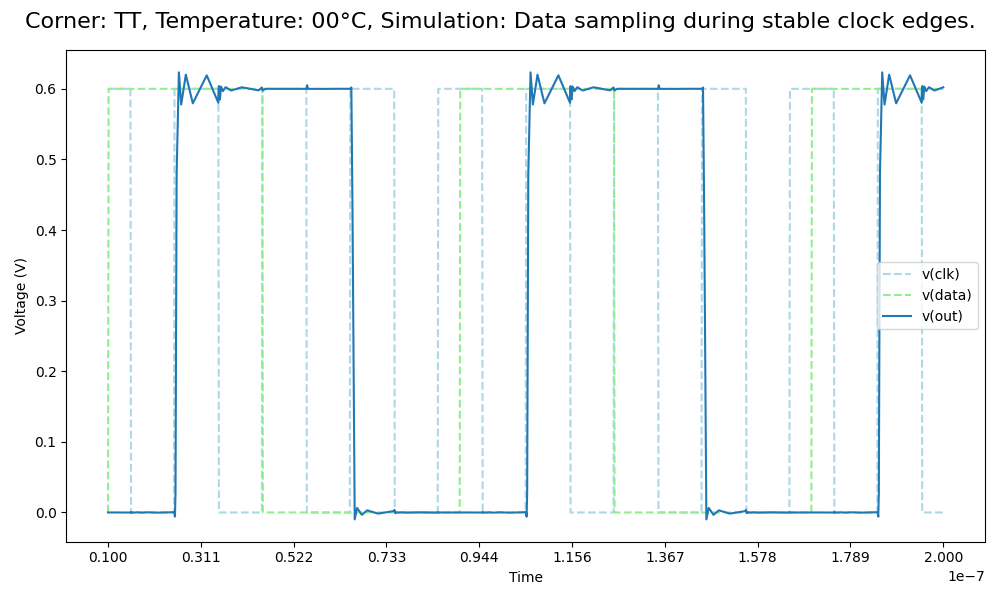
\includegraphics[height= 0.21\textheight]{figures/aimspice/0.600_0.1u_0.1u_0.3u_0.1u/functionality/TT00W2.png}
    \vspace{5pt}
    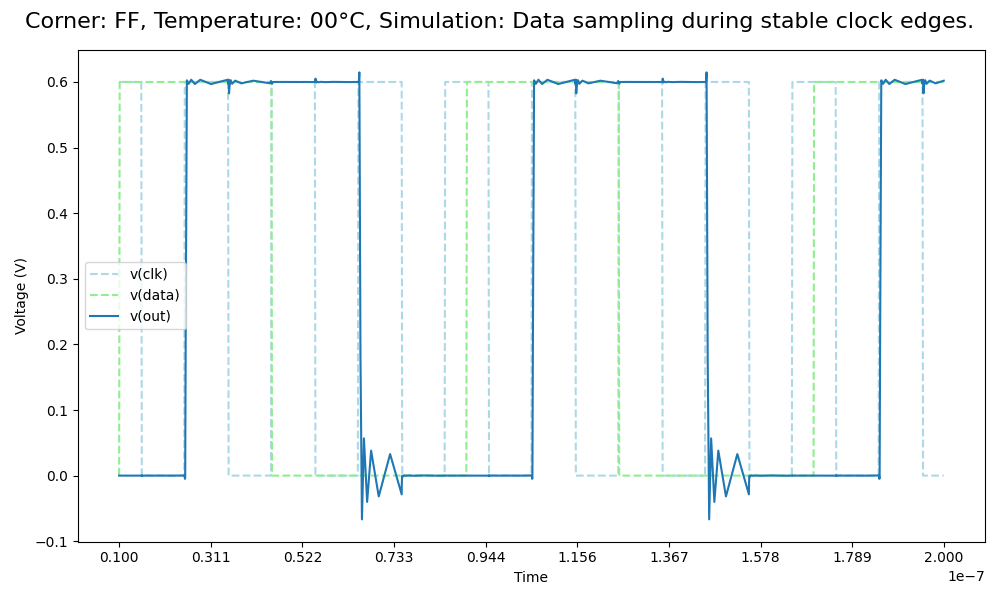
\includegraphics[height= 0.21\textheight]{figures/aimspice/0.600_0.1u_0.1u_0.3u_0.1u/functionality/FF00W2.png}
    \vspace{5pt}
    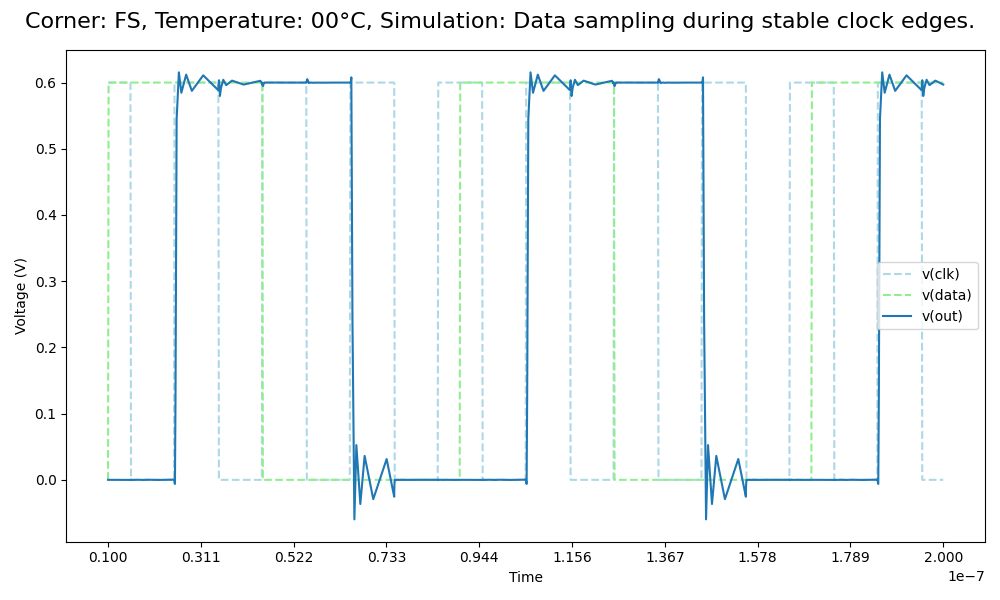
\includegraphics[height= 0.21\textheight]{figures/aimspice/0.600_0.1u_0.1u_0.3u_0.1u/functionality/FS00W2.png}
    \vspace{5pt}
    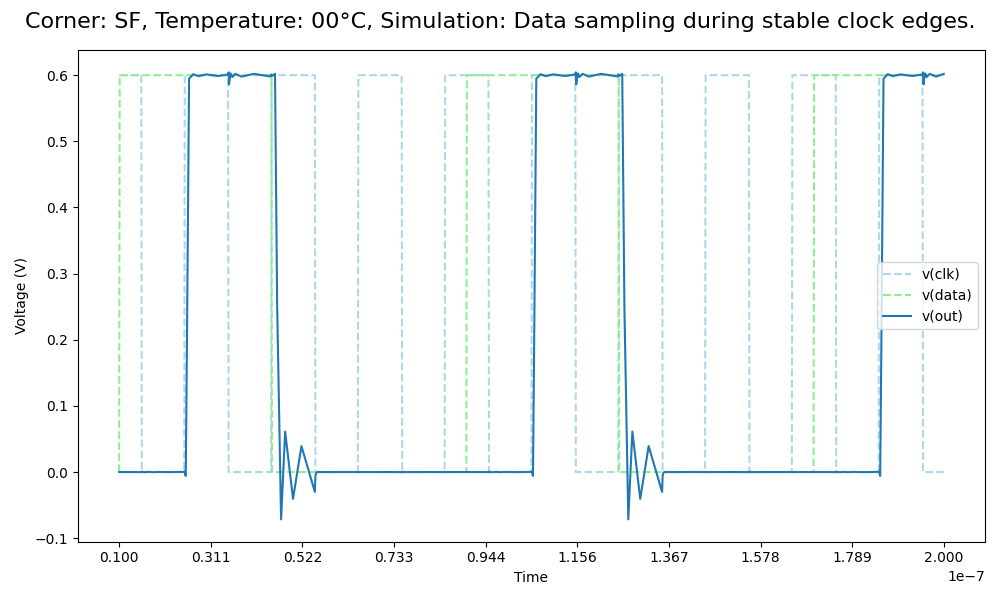
\includegraphics[height= 0.21\textheight]{figures/aimspice/0.600_0.1u_0.1u_0.3u_0.1u/functionality/SF00W2.png}
    \vspace{5pt}
    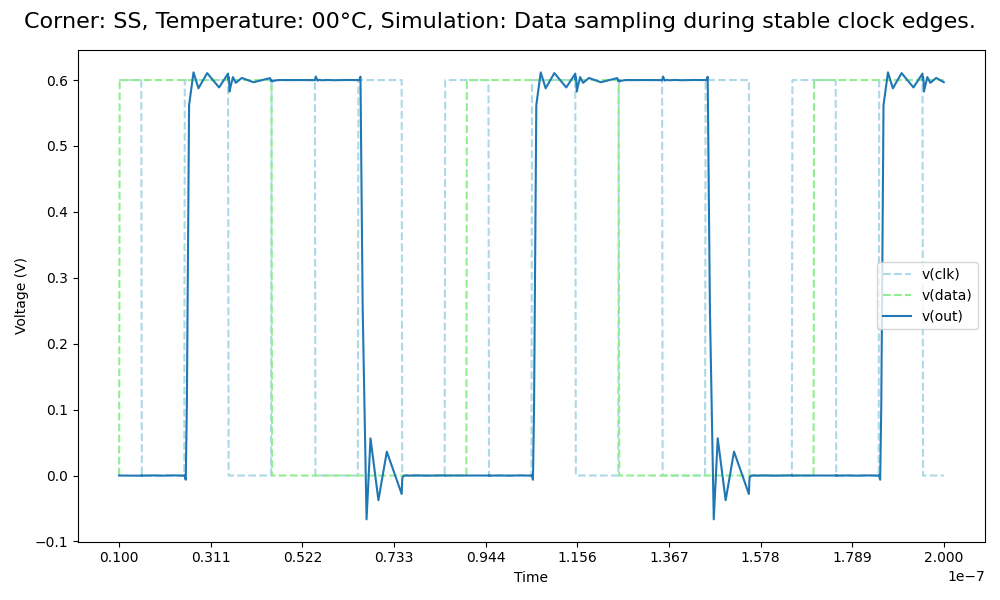
\includegraphics[height= 0.21\textheight]{figures/aimspice/0.600_0.1u_0.1u_0.3u_0.1u/functionality/SS00W2.png}
    \caption{Simulation of datasampling when the data stays the same for a few clock edges at 0 degrees celcius.}
    \label{fig:aimspice_W2_0}
\end{figure}

\pagebreak

\begin{figure}[H]
    \centering
    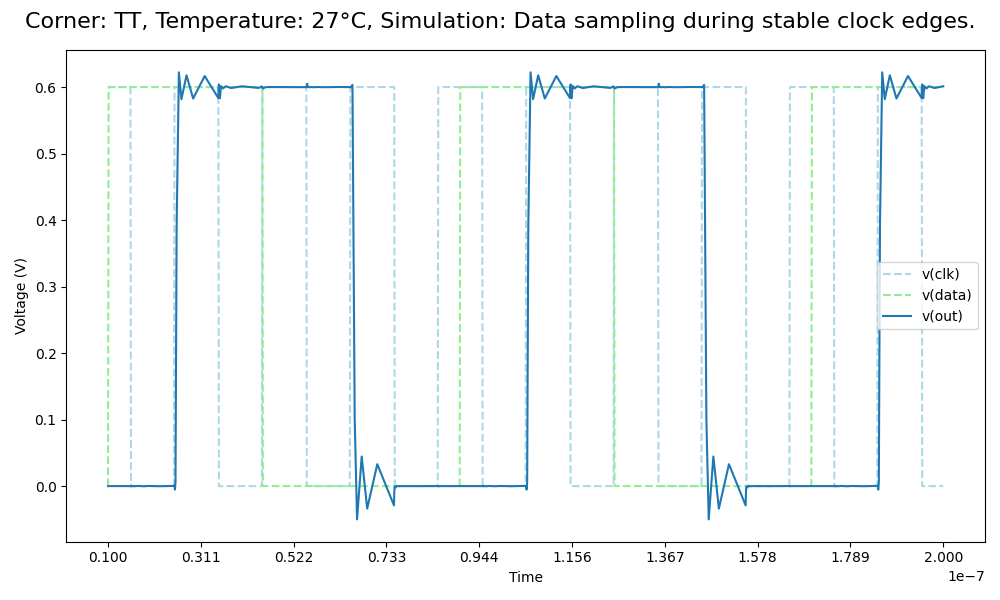
\includegraphics[height= 0.21\textheight]{figures/aimspice/0.600_0.1u_0.1u_0.3u_0.1u/functionality/TT27W2.png}
    \vspace{5pt}
    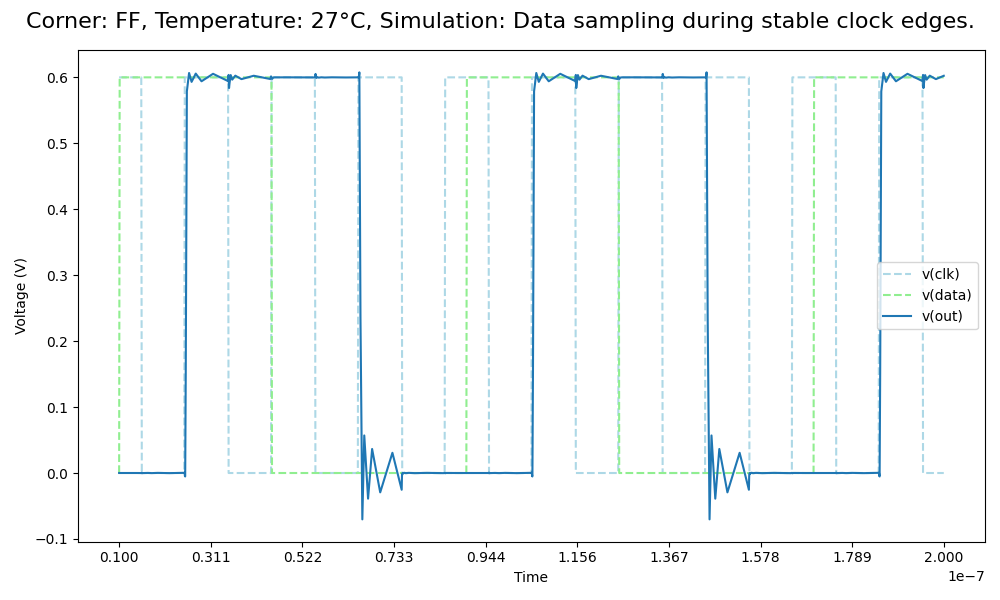
\includegraphics[height= 0.21\textheight]{figures/aimspice/0.600_0.1u_0.1u_0.3u_0.1u/functionality/FF27W2.png}
    \vspace{5pt}
    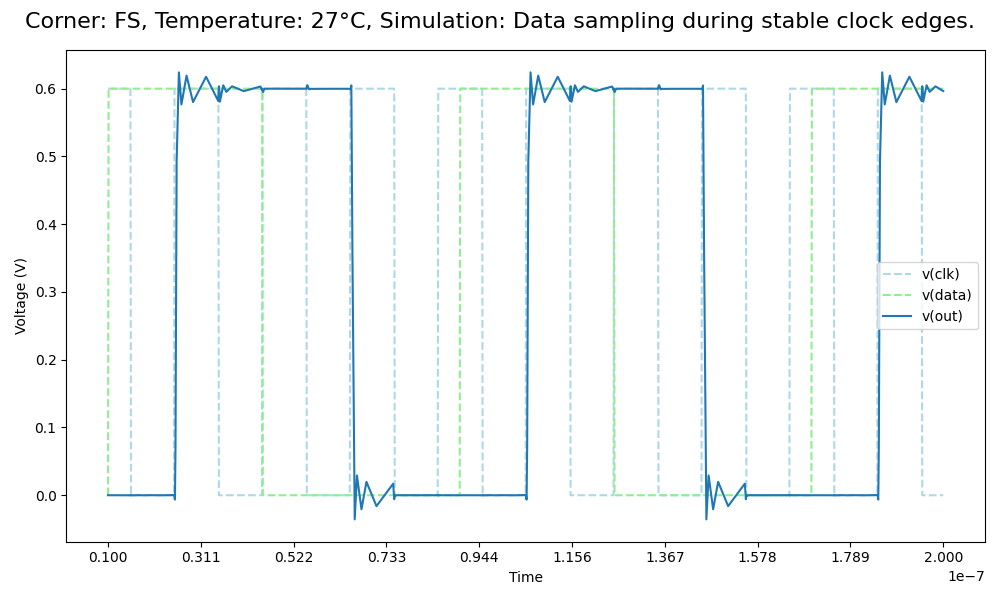
\includegraphics[height= 0.21\textheight]{figures/aimspice/0.600_0.1u_0.1u_0.3u_0.1u/functionality/FS27W2.png}
    \vspace{5pt}
    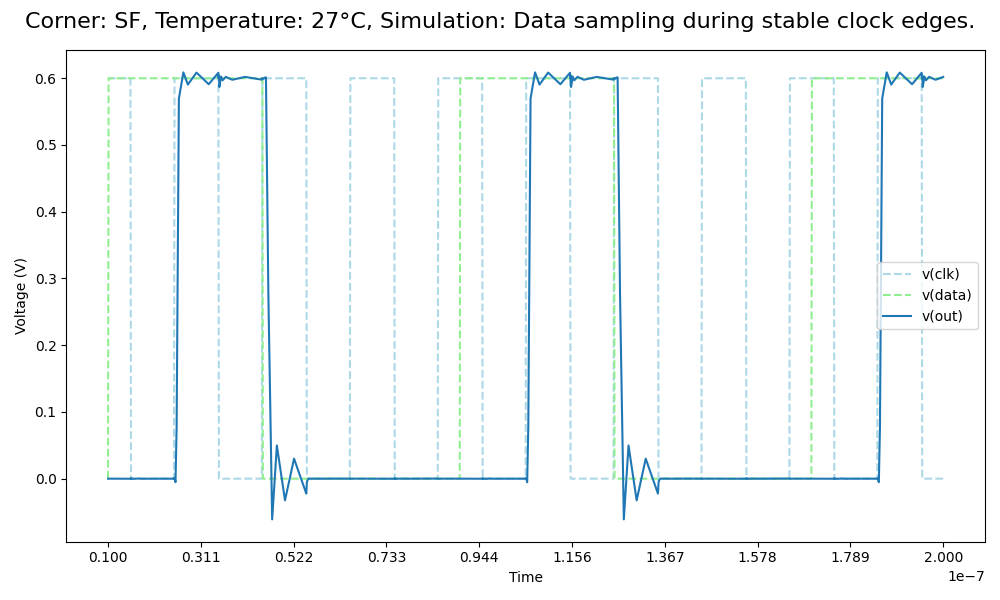
\includegraphics[height= 0.21\textheight]{figures/aimspice/0.600_0.1u_0.1u_0.3u_0.1u/functionality/SF27W2.png}
    \vspace{5pt}
    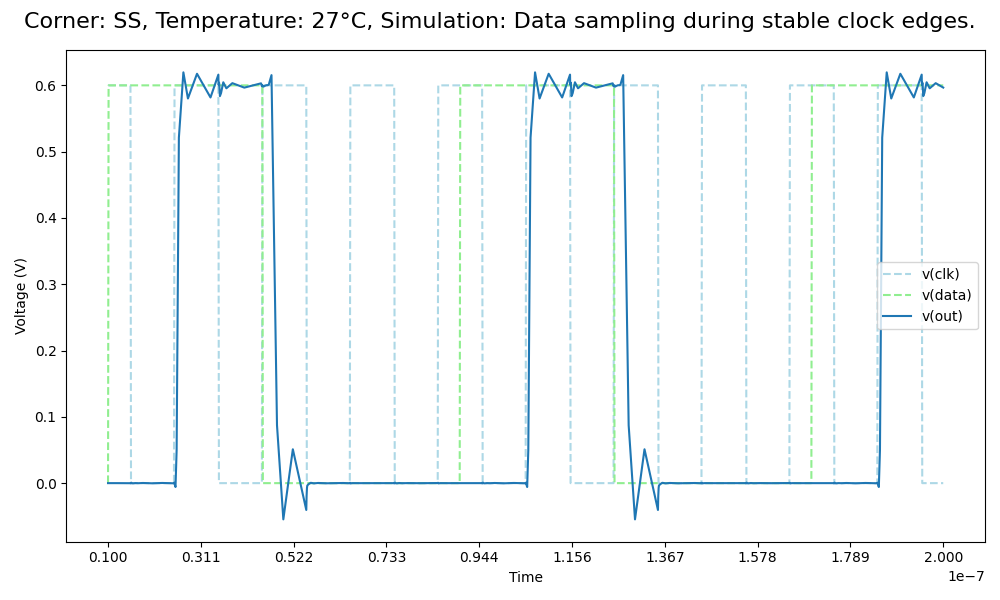
\includegraphics[height= 0.21\textheight]{figures/aimspice/0.600_0.1u_0.1u_0.3u_0.1u/functionality/SS27W2.png}
    \caption{Simulation of datasampling when the data stays the same for a few clock edges at 27 degrees celcius.}
    \label{fig:aimspice_W2_27}
\end{figure}

\pagebreak

\begin{figure}[H]
    \centering
    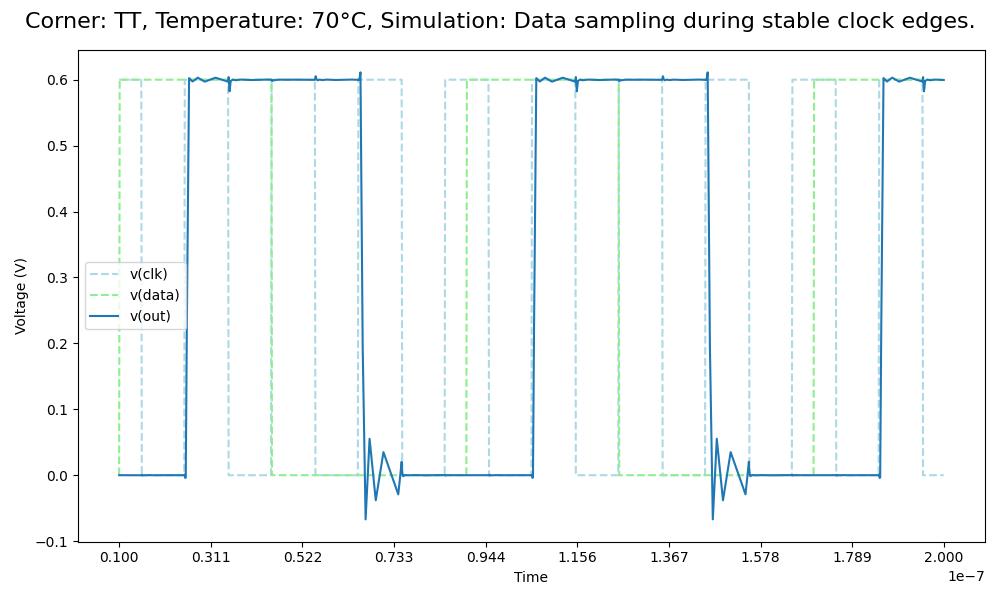
\includegraphics[height= 0.21\textheight]{figures/aimspice/0.600_0.1u_0.1u_0.3u_0.1u/functionality/TT70W2.png}
    \vspace{5pt}
    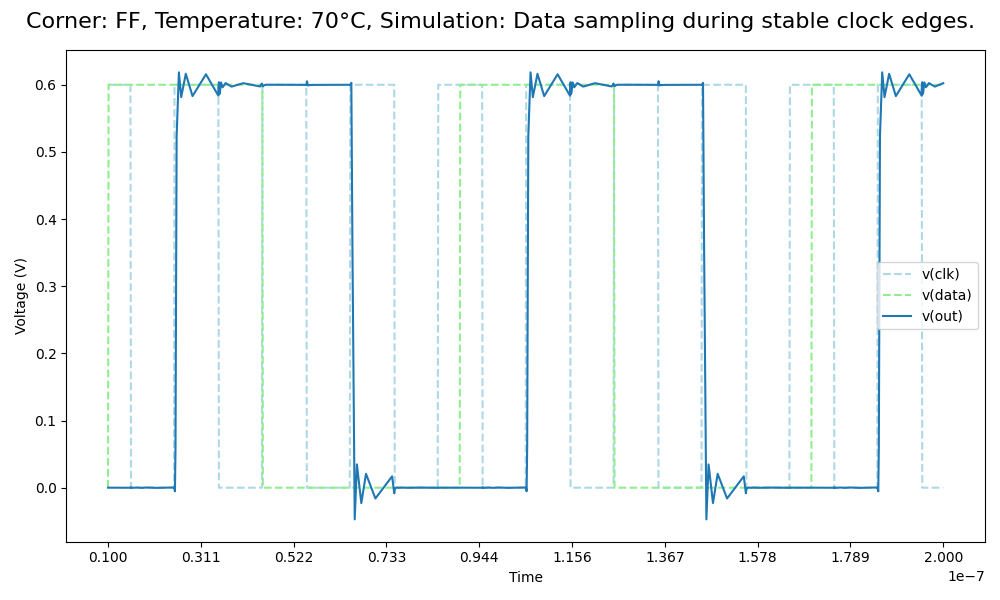
\includegraphics[height= 0.21\textheight]{figures/aimspice/0.600_0.1u_0.1u_0.3u_0.1u/functionality/FF70W2.png}
    \vspace{5pt}
    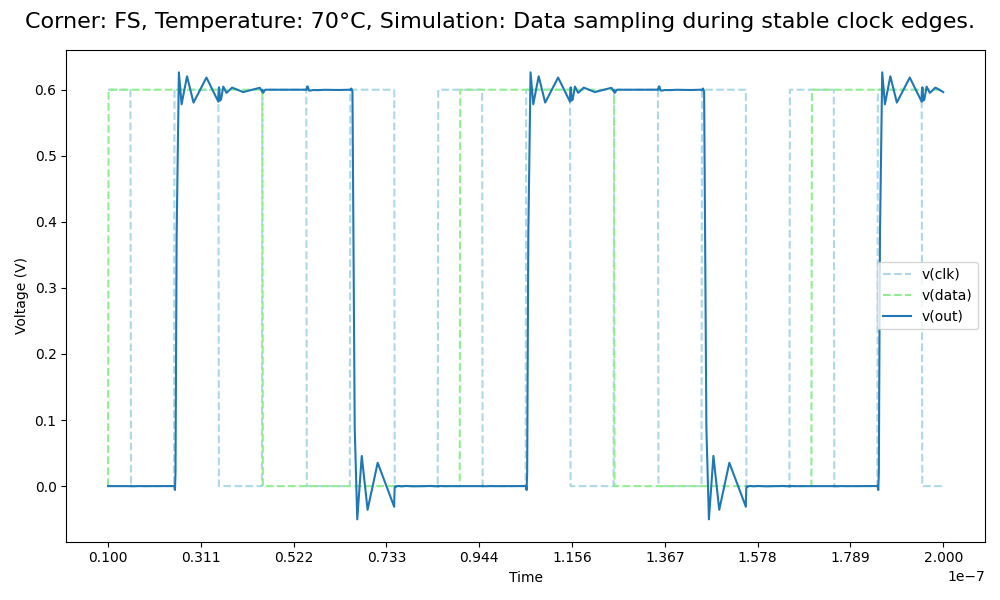
\includegraphics[height= 0.21\textheight]{figures/aimspice/0.600_0.1u_0.1u_0.3u_0.1u/functionality/FS70W2.png}
    \vspace{5pt}
    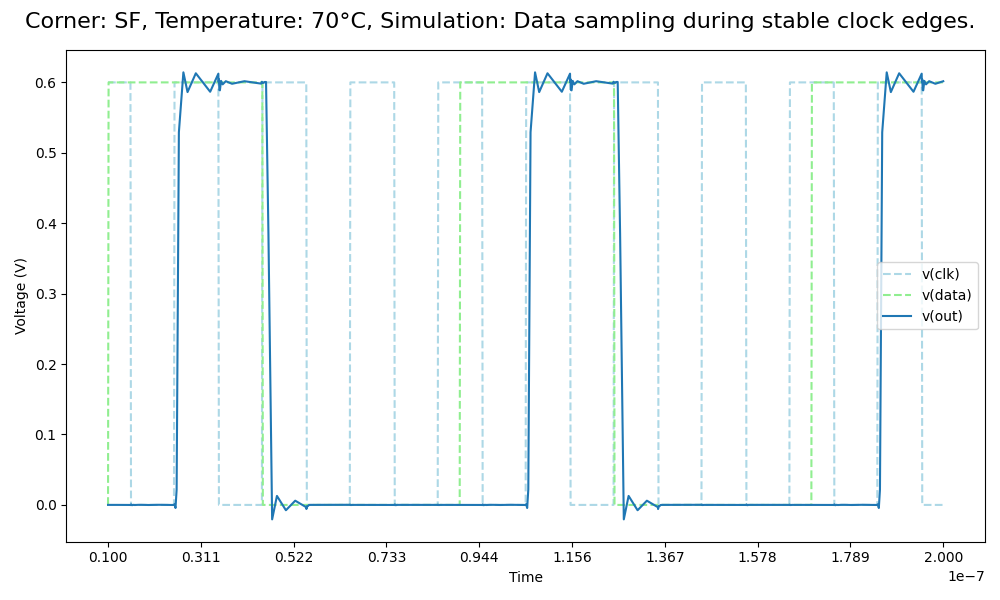
\includegraphics[height= 0.21\textheight]{figures/aimspice/0.600_0.1u_0.1u_0.3u_0.1u/functionality/SF70W2.png}
    \vspace{5pt}
    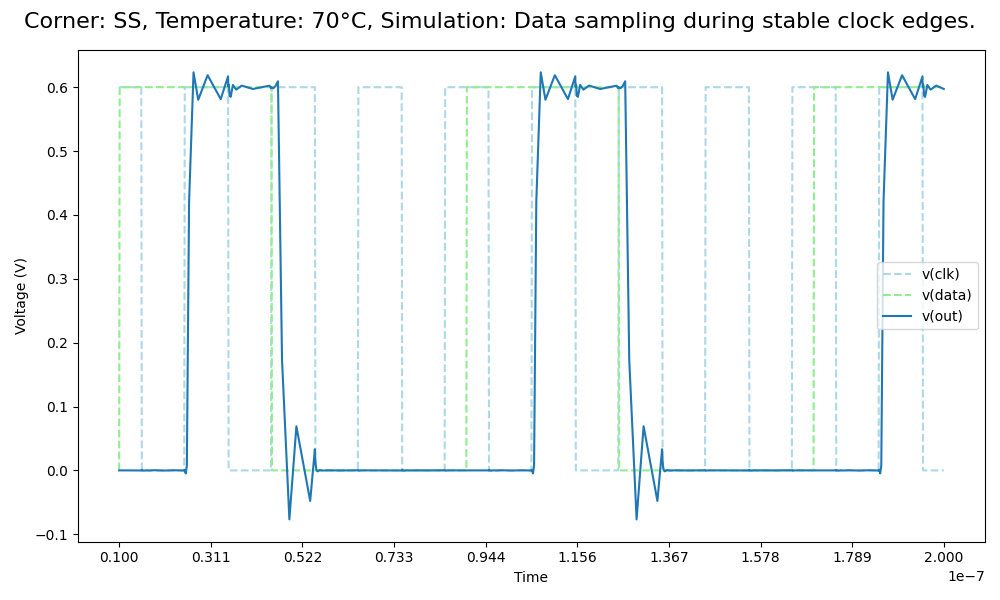
\includegraphics[height= 0.21\textheight]{figures/aimspice/0.600_0.1u_0.1u_0.3u_0.1u/functionality/SS70W2.png}
    \caption{Simulation of datasampling when the data stays the same for a few clock edges at 70 degrees celcius.}
    \label{fig:aimspice_W2_70}
\end{figure}

\pagebreak

\pagebreak

\begin{figure}[H]
    \centering
    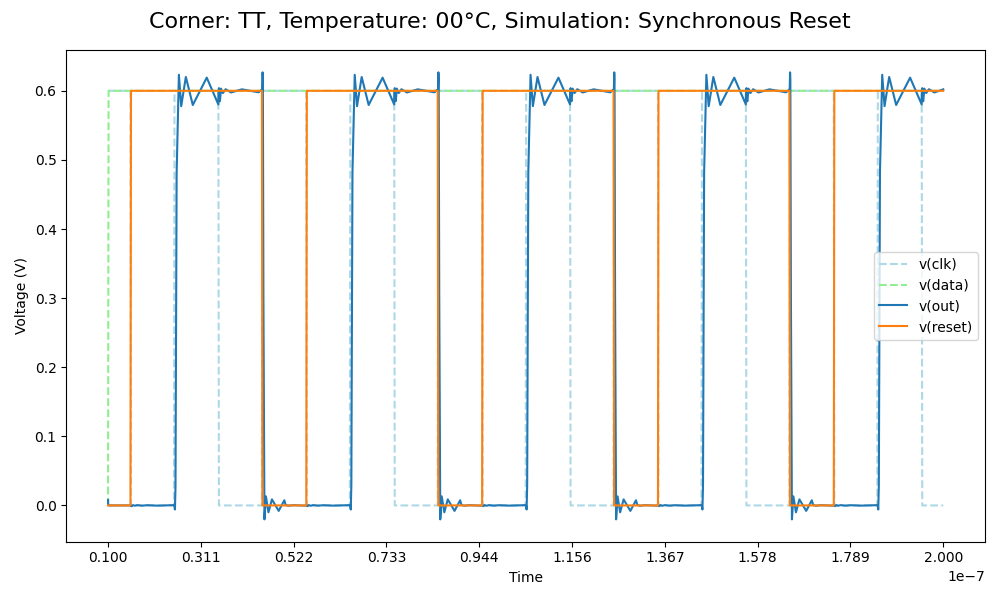
\includegraphics[height= 0.21\textheight]{figures/aimspice/0.600_0.1u_0.1u_0.3u_0.1u/functionality/TT00W3.png}
    \vspace{5pt}
    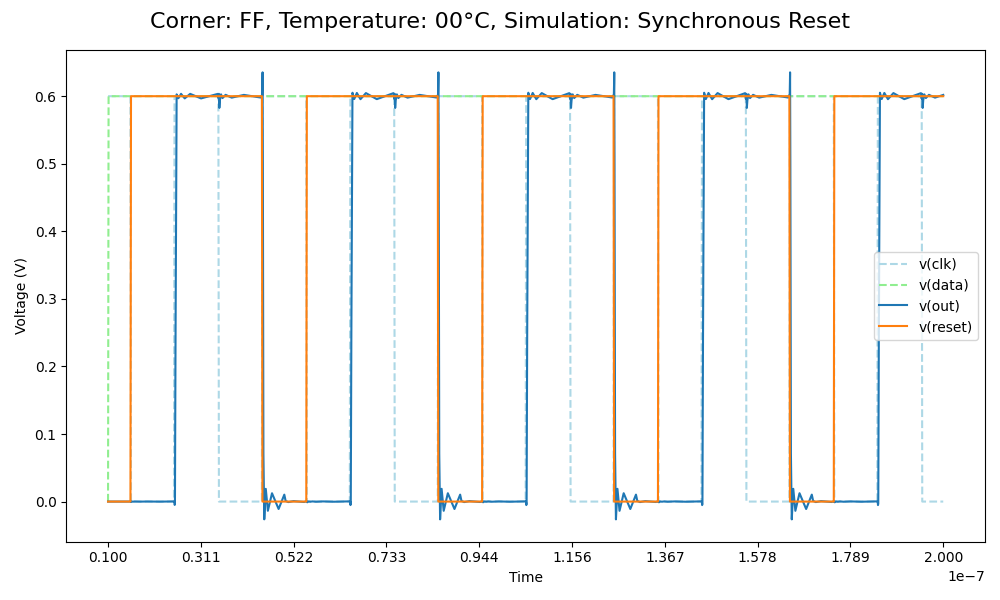
\includegraphics[height= 0.21\textheight]{figures/aimspice/0.600_0.1u_0.1u_0.3u_0.1u/functionality/FF00W3.png}
    \vspace{5pt}
    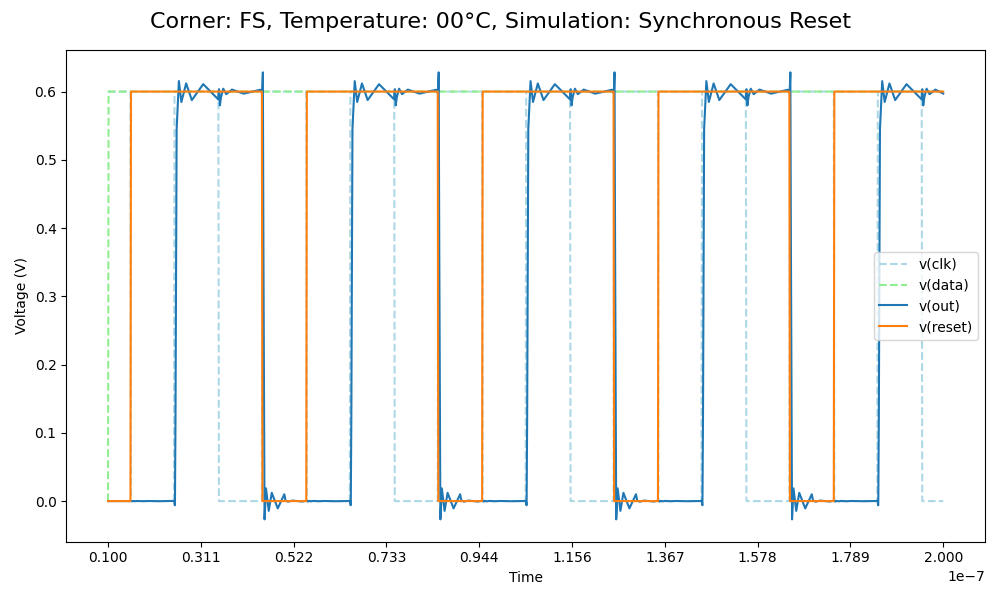
\includegraphics[height= 0.21\textheight]{figures/aimspice/0.600_0.1u_0.1u_0.3u_0.1u/functionality/FS00W3.png}
    \vspace{5pt}
    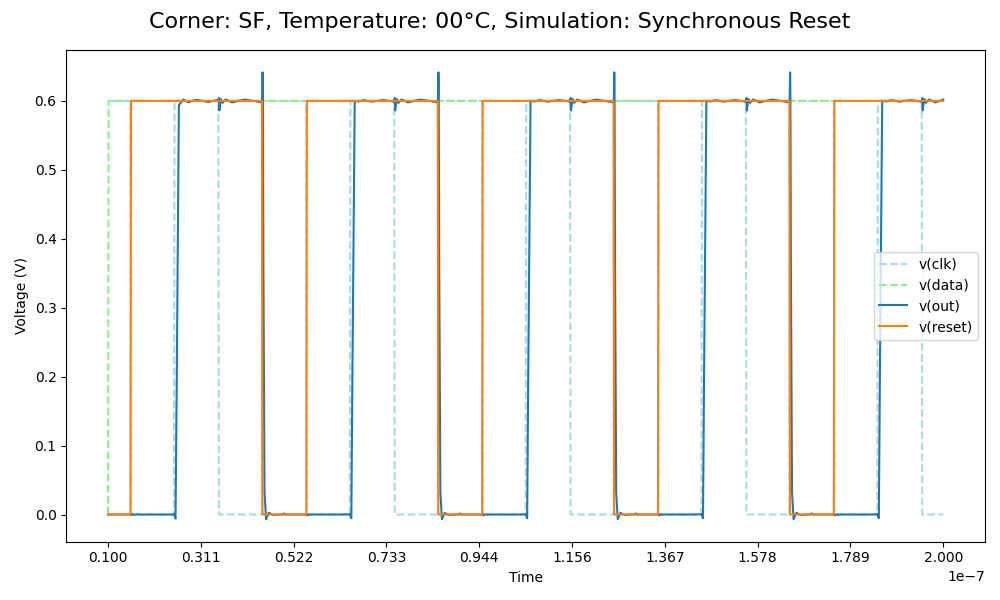
\includegraphics[height= 0.21\textheight]{figures/aimspice/0.600_0.1u_0.1u_0.3u_0.1u/functionality/SF00W3.png}
    \vspace{5pt}
    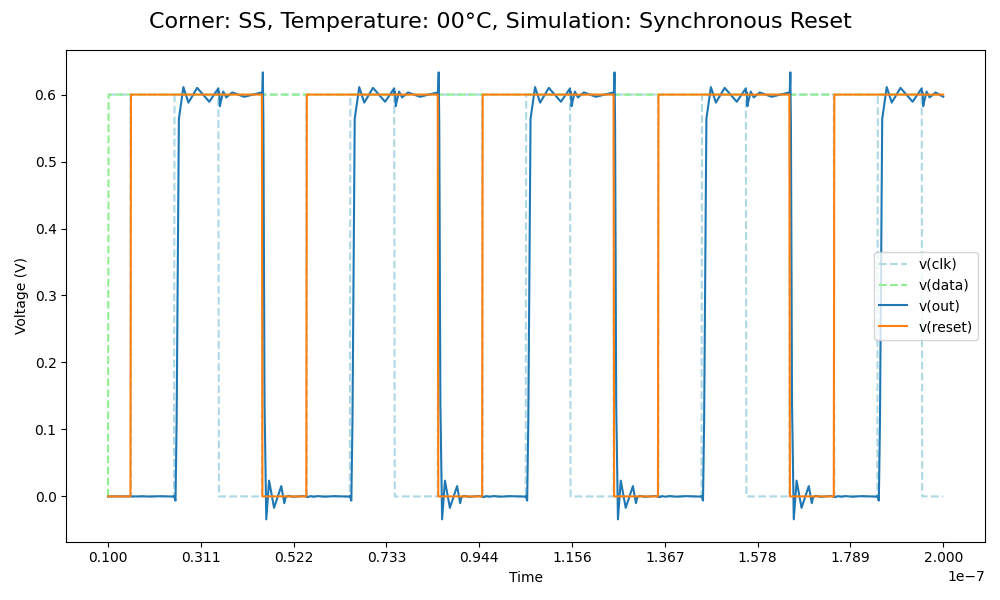
\includegraphics[height= 0.21\textheight]{figures/aimspice/0.600_0.1u_0.1u_0.3u_0.1u/functionality/SS00W3.png}
    \caption{Simulation of the reset at 0 degrees celcius.}
    \label{fig:aimspice_W3_0}
\end{figure}

\pagebreak

\begin{figure}[H]
    \centering
    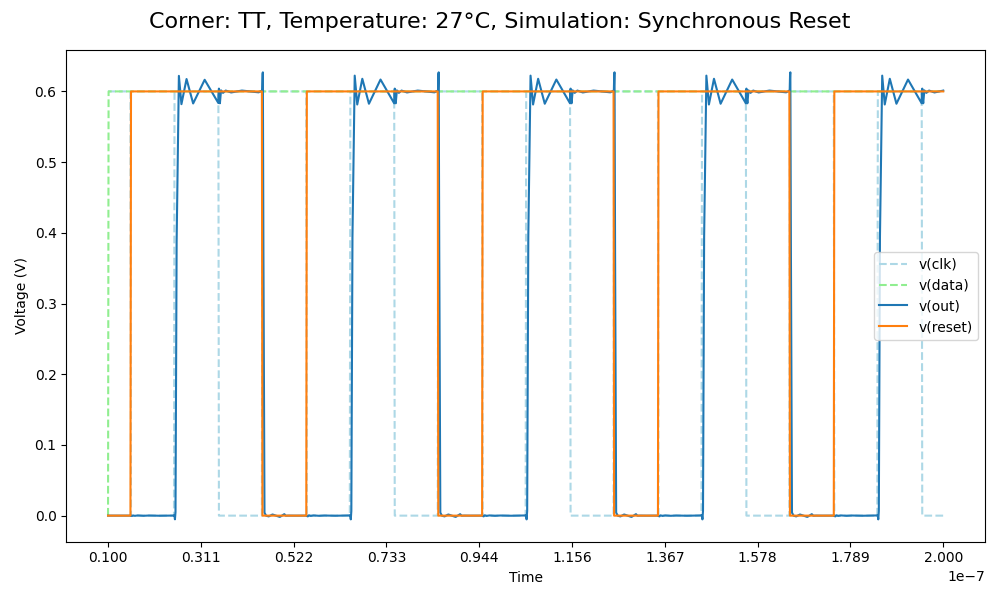
\includegraphics[height= 0.21\textheight]{figures/aimspice/0.600_0.1u_0.1u_0.3u_0.1u/functionality/TT27W3.png}
    \vspace{5pt}
    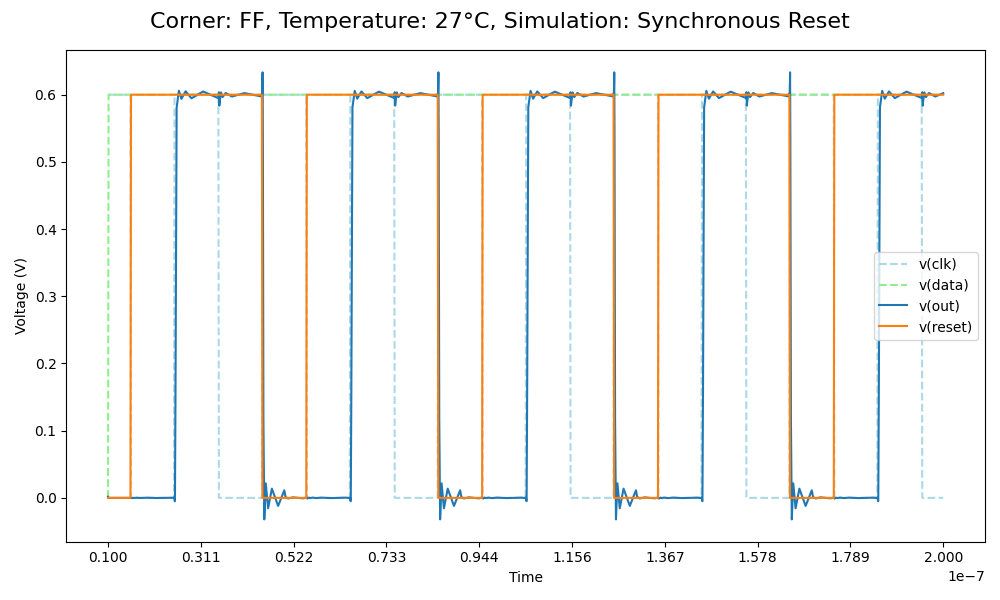
\includegraphics[height= 0.21\textheight]{figures/aimspice/0.600_0.1u_0.1u_0.3u_0.1u/functionality/FF27W3.png}
    \vspace{5pt}
    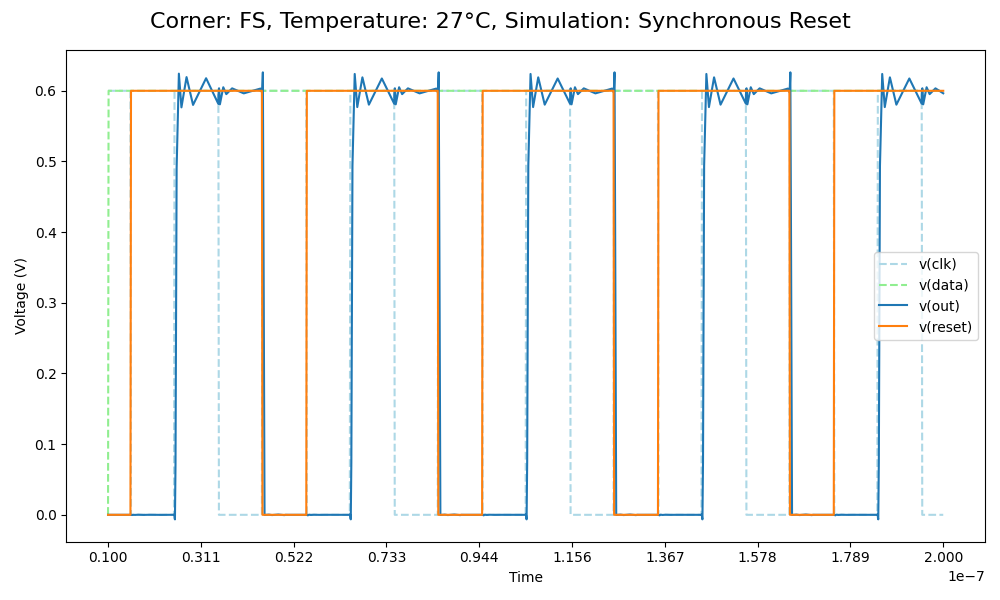
\includegraphics[height= 0.21\textheight]{figures/aimspice/0.600_0.1u_0.1u_0.3u_0.1u/functionality/FS27W3.png}
    \vspace{5pt}
    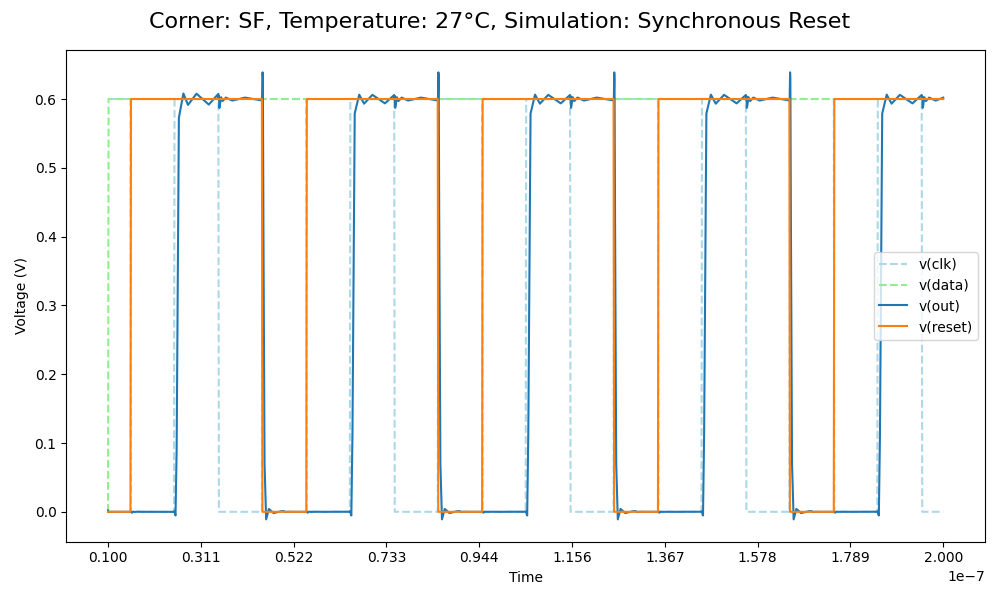
\includegraphics[height= 0.21\textheight]{figures/aimspice/0.600_0.1u_0.1u_0.3u_0.1u/functionality/SF27W3.png}
    \vspace{5pt}
    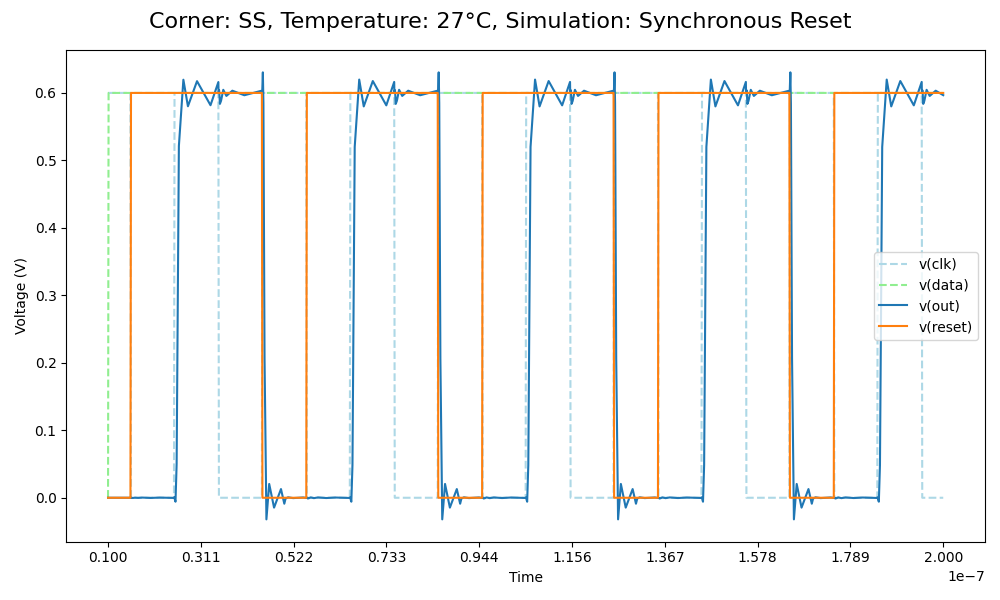
\includegraphics[height= 0.21\textheight]{figures/aimspice/0.600_0.1u_0.1u_0.3u_0.1u/functionality/SS27W3.png}
    \caption{Simulation of the reset at 27 degrees celcius.}
    \label{fig:aimspice_W3_27}
\end{figure}

\pagebreak

\begin{figure}[H]
    \centering
    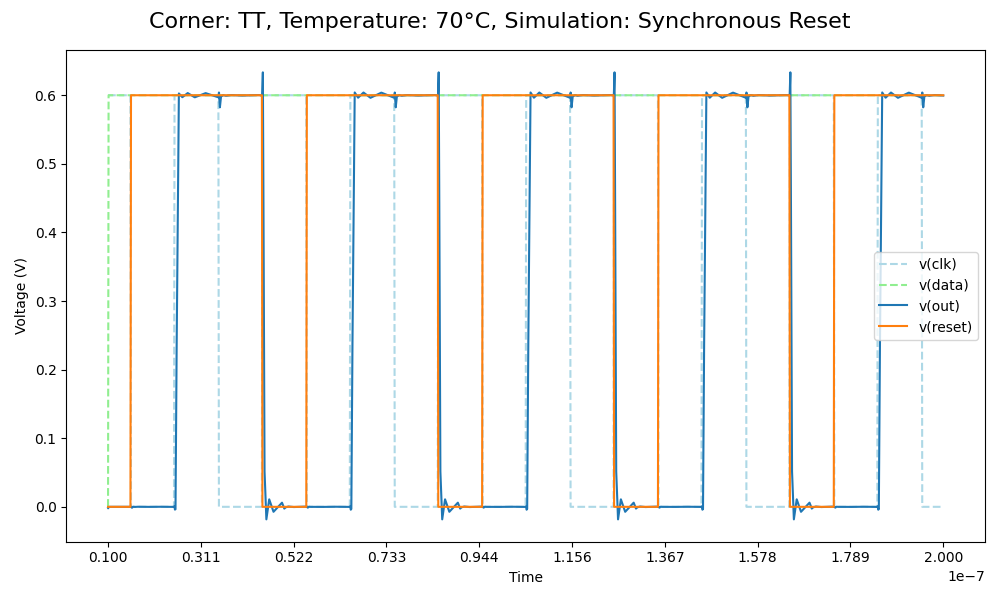
\includegraphics[height= 0.21\textheight]{figures/aimspice/0.600_0.1u_0.1u_0.3u_0.1u/functionality/TT70W3.png}
    \vspace{5pt}
    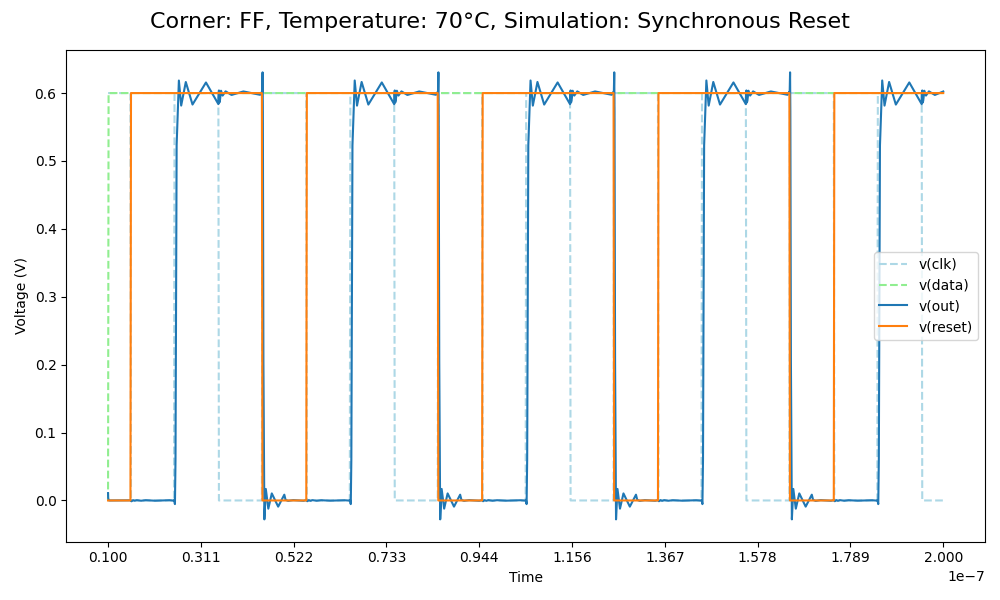
\includegraphics[height= 0.21\textheight]{figures/aimspice/0.600_0.1u_0.1u_0.3u_0.1u/functionality/FF70W3.png}
    \vspace{5pt}
    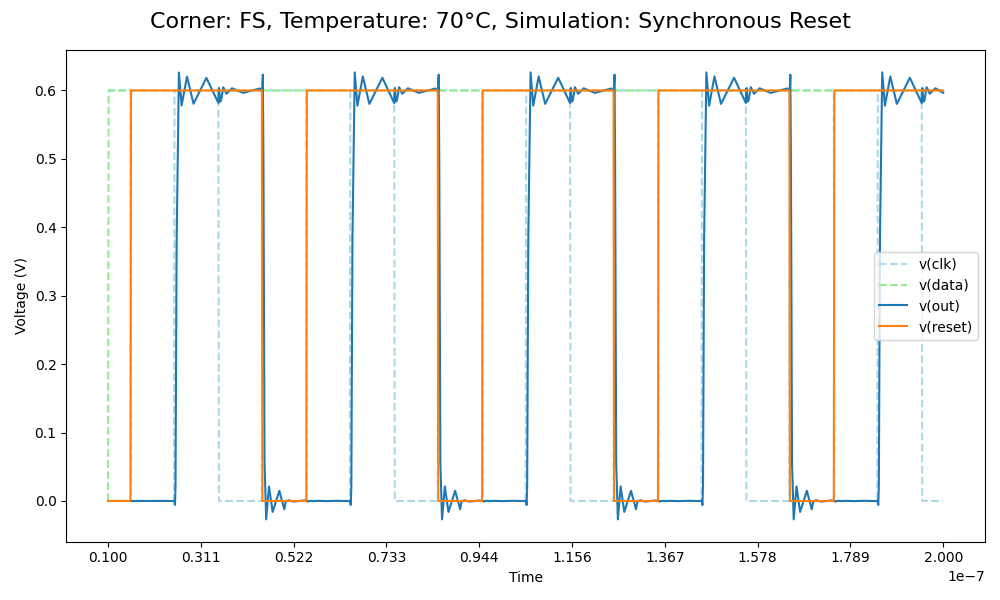
\includegraphics[height= 0.21\textheight]{figures/aimspice/0.600_0.1u_0.1u_0.3u_0.1u/functionality/FS70W3.png}
    \vspace{5pt}
    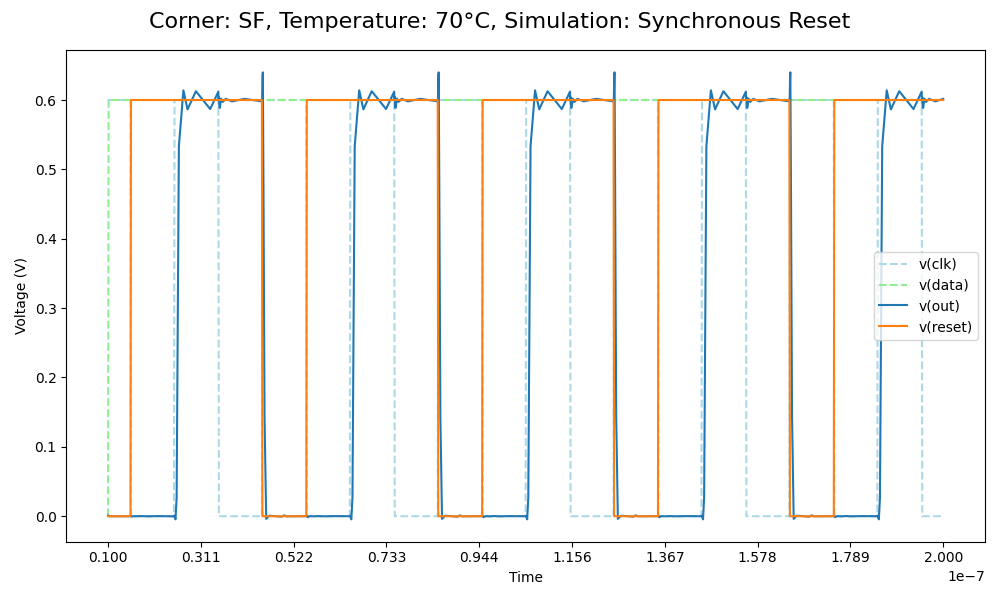
\includegraphics[height= 0.21\textheight]{figures/aimspice/0.600_0.1u_0.1u_0.3u_0.1u/functionality/SF70W3.png}
    \vspace{5pt}
    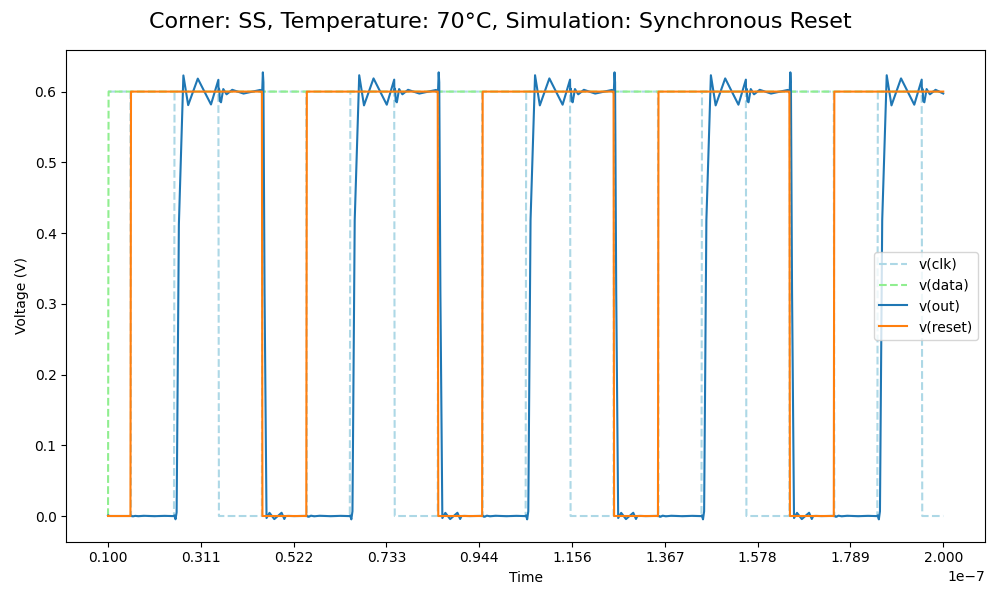
\includegraphics[height= 0.21\textheight]{figures/aimspice/0.600_0.1u_0.1u_0.3u_0.1u/functionality/SS70W3.png}
    \caption{Simulation of the reset at 70 degrees celcius.}
    \label{fig:aimspice_W3_70}
\end{figure}

The computed static leakage power with respect to the chosen $V_{DD}\pm 0.2V$ and with respect to the chosen $W_P$ can be seen in the figures \ref{fig:0.3_I1_I2}, \ref{fig:0.3_I3_I4} \ref{fig:0.6_I1_I2} and \ref{fig:0.6_I3_I4}. The dotes are the actual values computed while the the lines are fitted line with a degree of 5 to aid in the visualisation of the trends regardig the variables.

\imagesidebyside{figures/aimspice/variableVDD/CSV/static_power_leakage_graph_I1.png}{I1}{figures/aimspice/variableVDD/CSV/static_power_leakage_graph_I2.png}{I2}{Static leakage power when  $W_N=0.1u$, $L_N=0.1u$, $P_W=0.3u$ and $L_P=0.1u$}{0.3_I1_I2}{0.49}

\imagesidebyside{figures/aimspice/variableVDD/CSV/static_power_leakage_graph_I3.png}{I3}{figures/aimspice/variableVDD/CSV/static_power_leakage_graph_I4.png}{I4}{Static leakage power when  $W_N=0.1u$, $L_N=0.1u$, $P_W=0.3u$ and $L_P=0.1u$}{0.3_I3_I4}{0.49}

\imagesidebyside{figures/aimspice/variableParam/CSV/static_power_leakage_graph_0.6_I1.png}{I1}{figures/aimspice/variableParam/CSV/static_power_leakage_graph_0.6_I2.png}{I2}{Static leakage power when $V_{DD}=0.6V$, $W_N=0.1u$, $L_N=0.1u$ and $L_P=0.1u$}{0.6_I1_I2}{0.49}

\imagesidebyside{figures/aimspice/variableParam/CSV/static_power_leakage_graph_0.6_I3.png}{I3}{figures/aimspice/variableParam/CSV/static_power_leakage_graph_0.6_I4.png}{I4}{Static leakage power when $V_{DD}=0.6V$, $W_N=0.1u$, $L_N=0.1u$ and $L_P=0.1u$}{0.6_I3_I4}{0.49}

The computed delays with respect to the chosen $V_{DD}\pm 0.2V$ and with respect to the chosen $W_P$ can be seen in the figures \ref{fig:0.3_delay}, \ref{fig:0.3_delay} \ref{fig:0.6_delay} and \ref{fig:0.6_delay}. The dotes are the actual values computed while the the lines are fitted line with a degree of 5 to aid in the visualisation of the trends regardig the variables.

\imagesidebyside{figures/aimspice/variableVDD/CSV_time/propagation_delays_graph.png}{Propagnation delay}{figures/aimspice/variableVDD/CSV_time/rise_fall_times_graph.png}{Rise and fall time}{Delay and times when $W_N=0.1u$, $L_N=0.1u$, $P_W=0.3u$ and $L_P=0.1u$}{0.6_delay}{0.49}

\imagesidebyside{figures/aimspice/variableParam/CSV_time/propagation_delays_graph.png}{Propagnation delay}{figures/aimspice/variableParam/CSV_time/rise_fall_times_graph.png}{Rise and fall time}{Delay and times when $V_{DD}=0.6V$, $W_N=0.1u$, $L_N=0.1u$ and $L_P=0.1u$}{0.3_delay}{0.49}